\documentclass{exam}

\usepackage{units} 
\usepackage{xfrac} 
\usepackage[fleqn]{amsmath}
\usepackage{cancel}
\usepackage{float}
\usepackage{mdwlist}
\usepackage{booktabs}
\usepackage{cancel}
\usepackage{polynom}
\usepackage{caption}
\usepackage{fullpage}
\usepackage{comment}
\usepackage{enumerate}
\usepackage{graphicx}

\everymath{\displaystyle}

\printanswers

\ifprintanswers 
  \usepackage{2in1, lscape} 
\fi

\author{}
\date{\today}
\title{Statistics \\ Homework Four}

\begin{document}

  \maketitle

  \ifprintanswers
  \else
    \begin{itemize*}
      \item read Chapter 4 
      \item answer the questions in ``Check Your Skills'' and check the answers in the
        back of the book
      \item hand in exercises TO DO
    \end{itemize*}
  \fi

  \ifprintanswers
    \begin{description}
      \item[25]     
        \begin{parts}
          \part yes
          \part One kid got a 10 out of 100 on the test but estimated himself as a 4 out
          of 5 reader.  
        \end{parts}
    
      \item[26]
        \begin{figure}[H]
          \centering
          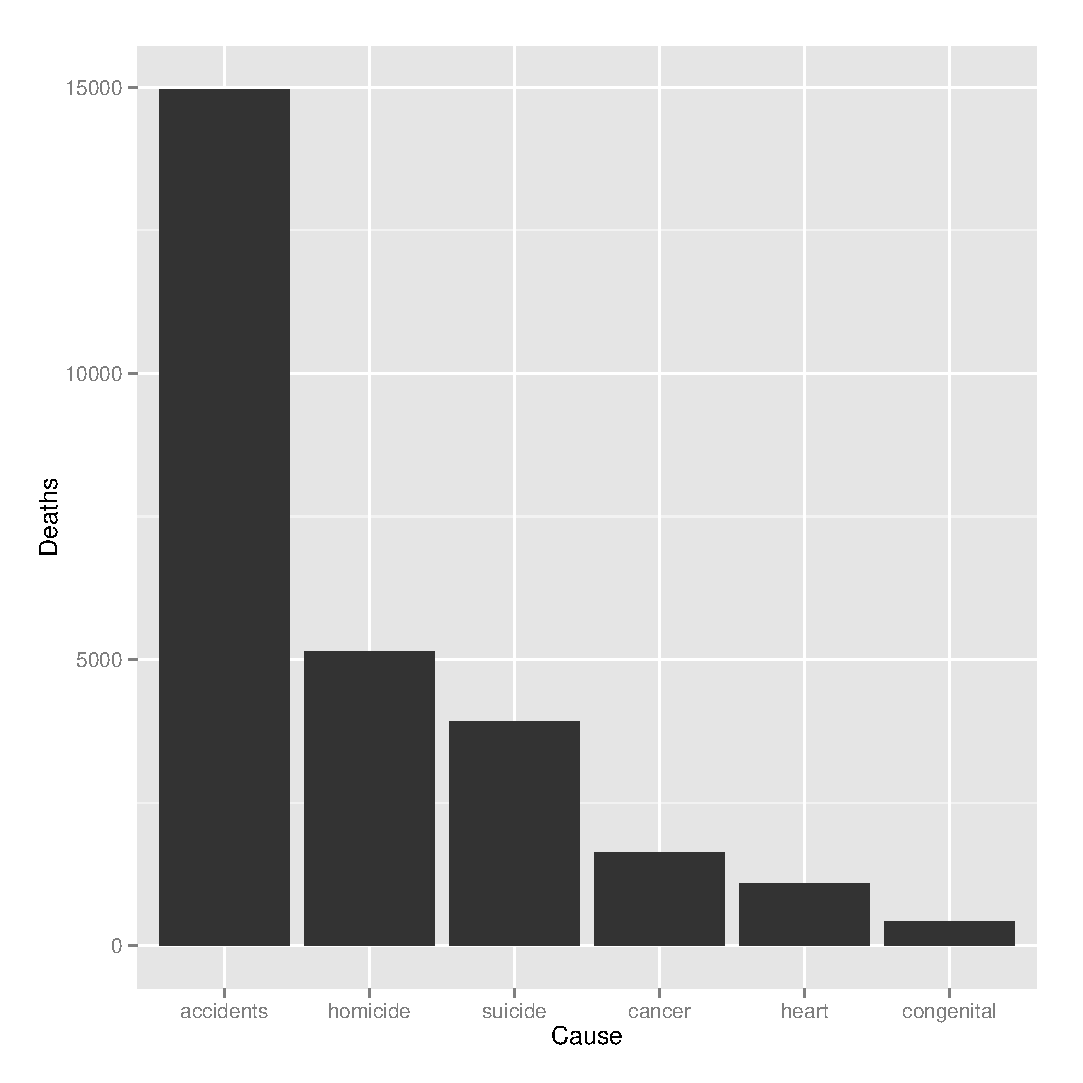
\includegraphics{figures/ex26.eps}
          \caption{Exercise 26}
        \end{figure}

        The correlation is 0.5653 so it looks like there is a mild preference
        for tall people to date each other.

      \item[27]
        \begin{parts}
          \part
            \begin{figure}[H]
              \centering
              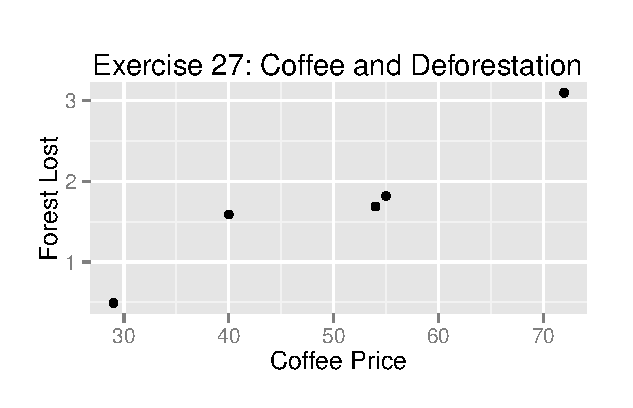
\includegraphics{figures/ex27.eps}
              \caption{Exercise 27}
            \end{figure}

          \part
            The correlation is 0.9552.  There is a strong correlation between the
            coffee price and deforestation.

          \part
            The units of the price don't matter.  Changing the currency would just
            change the labels on the y axis.

        \end{parts}

      \item[28]
        \begin{figure}[H]
          \centering
          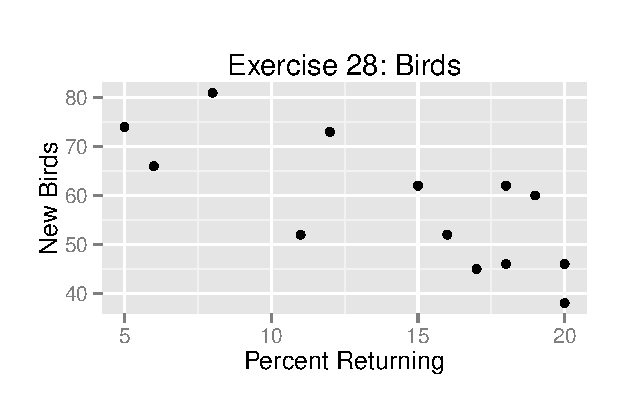
\includegraphics{figures/ex28.eps}
          \caption{Exercise 28}
        \end{figure}

        \begin{parts}
          \part
            The correlation is -0.7485.  There is a fairly strong negative correlation 
            between the number of birds that come back and the number of new birds.

            There probably isn't any room for new birds when large numbers of returning
            birds take up all the space.

          \part
            The sparrowhalk seems to be a long-lived territorial bird.

        \end{parts}

    \end{description}


  \else
    \vspace{11 cm}
    \begin{quote}
      \begin{em}
        Even voting for the right is doing nothing for it. It is only expressing to men
        feebly your desire that it should prevail. 
        % A wise man will not leave the right to the mercy of chance, nor wish it to
        % prevail through the power of the majority. There is but little virtue in the
        % action of masses of men. When the majority shall at length vote for the
        % abolition of slavery, it will be because they are indifferent to slavery, or
        % because there is but little slavery left to be abolished by their vote. 
      \end{em}
    \end{quote}
    \hspace{1 cm} --Henry David Thoreau
  \fi

\end{document}

